\documentclass[../main.tex]{subfiles}
\begin{document}

\chapter{Solcellesystem} \label{Chap:Solcellesystem}
Solcelle-delen er den primære leverandør af energi til systemet. Det er derfor vigtigt at vi får mest mulig effekt ud af den. Følgende afsnit beskriver hvordan dette er opnået. Først og fremmest måles spændingen og strømmen leveret af solcellen. Derefter behandler et MPPT-system værdierne og sørger for at spændinger og strømme reguleres til give størst effekt. Til sidst sidder en buck-konverter som sørger for en konstant 5V spænding til energilageret.

\subsection{MPPT strøm/spændingsmåler}
    Måle-kredsløbet der sidder på solcellens udgang bruges til at måle dens udgangsstrøm og spænding. Denne information skal bruges af arduionen, som sørger for at værdierne bruges så optimalt som muligt og systemet får mest muligt effekt ud af solcellen.
            
        \subsubsection{Delkrav}

        \begin{enumerate}
                \item Måle-kredsløbet skal implementeres med diskrete komponenter - ingen integreret kredsløb med undtagelse af op-amps.
        \end{enumerate}
        
        \subsubsection{Designovervejelser}
        Strømmålingen kan realiseres ved en såkaldt shunt-modstand. Princippet bag denne er, at man ønsker en meget lille modstand som man kan måle spændingen over, og derved udregne strømmen der løber igennem den. Da spændingen over den kommer til at være meget lille, kan en op-amp integreres i kredsløbet til at forstærke værdien op.

        Spændingsmålingen kan laves ved en simpel spændingsdeler. Men da vi allerede bruger en MCP6002 chip med 2 op-amps i, valgte vi at bruge den anden til spændingsmålingen.
            
        \subsubsection{Implementering}

        En effektmodstand på 0,1 ohm er brugt til strømmålingen, hvorefter spændingen over den ganges op med en faktor 75 gennem et op-amp differenskoblingstrin. På den måde sikre vi at den maksimale indgangsstrøm til arduionen ikke overstiger 5V, da det er den højest mulige strøm ganget forstærkningen der kan leveres.

        Spændingsmåleren måler over en spændingsdeler som forstærkes 2,26/10-dele. Derved vil den højest mulige spænding fra solcellen maksimalt være 5V på Arduionens indgang.

        Måle-kredsløbet er vist nedenfor. 
        

        \begin{figure}[H]
        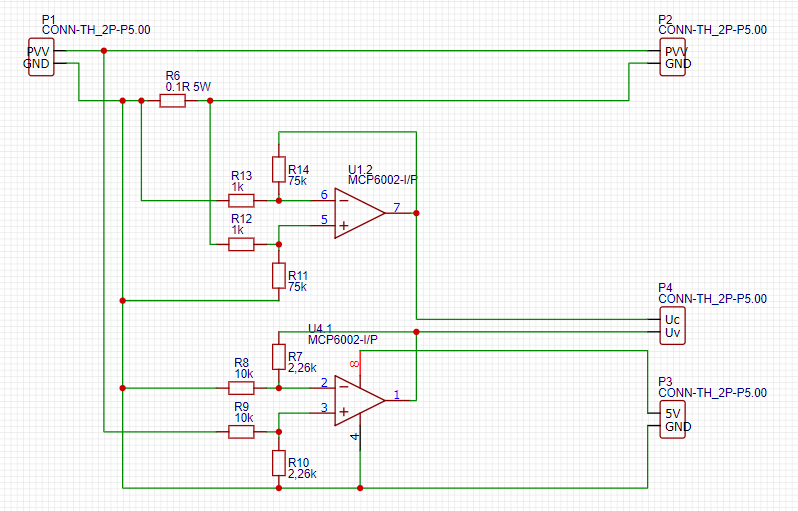
\includegraphics[width=\textwidth]{Dokumentation/målekredsløb.png}
        \caption{Strøm- og spændingsmåler kredsløb}
        \label{fig: Strøm- og spændingsmåler kredsløb}
        \end{figure}
        
        \begin{figure}[H]
        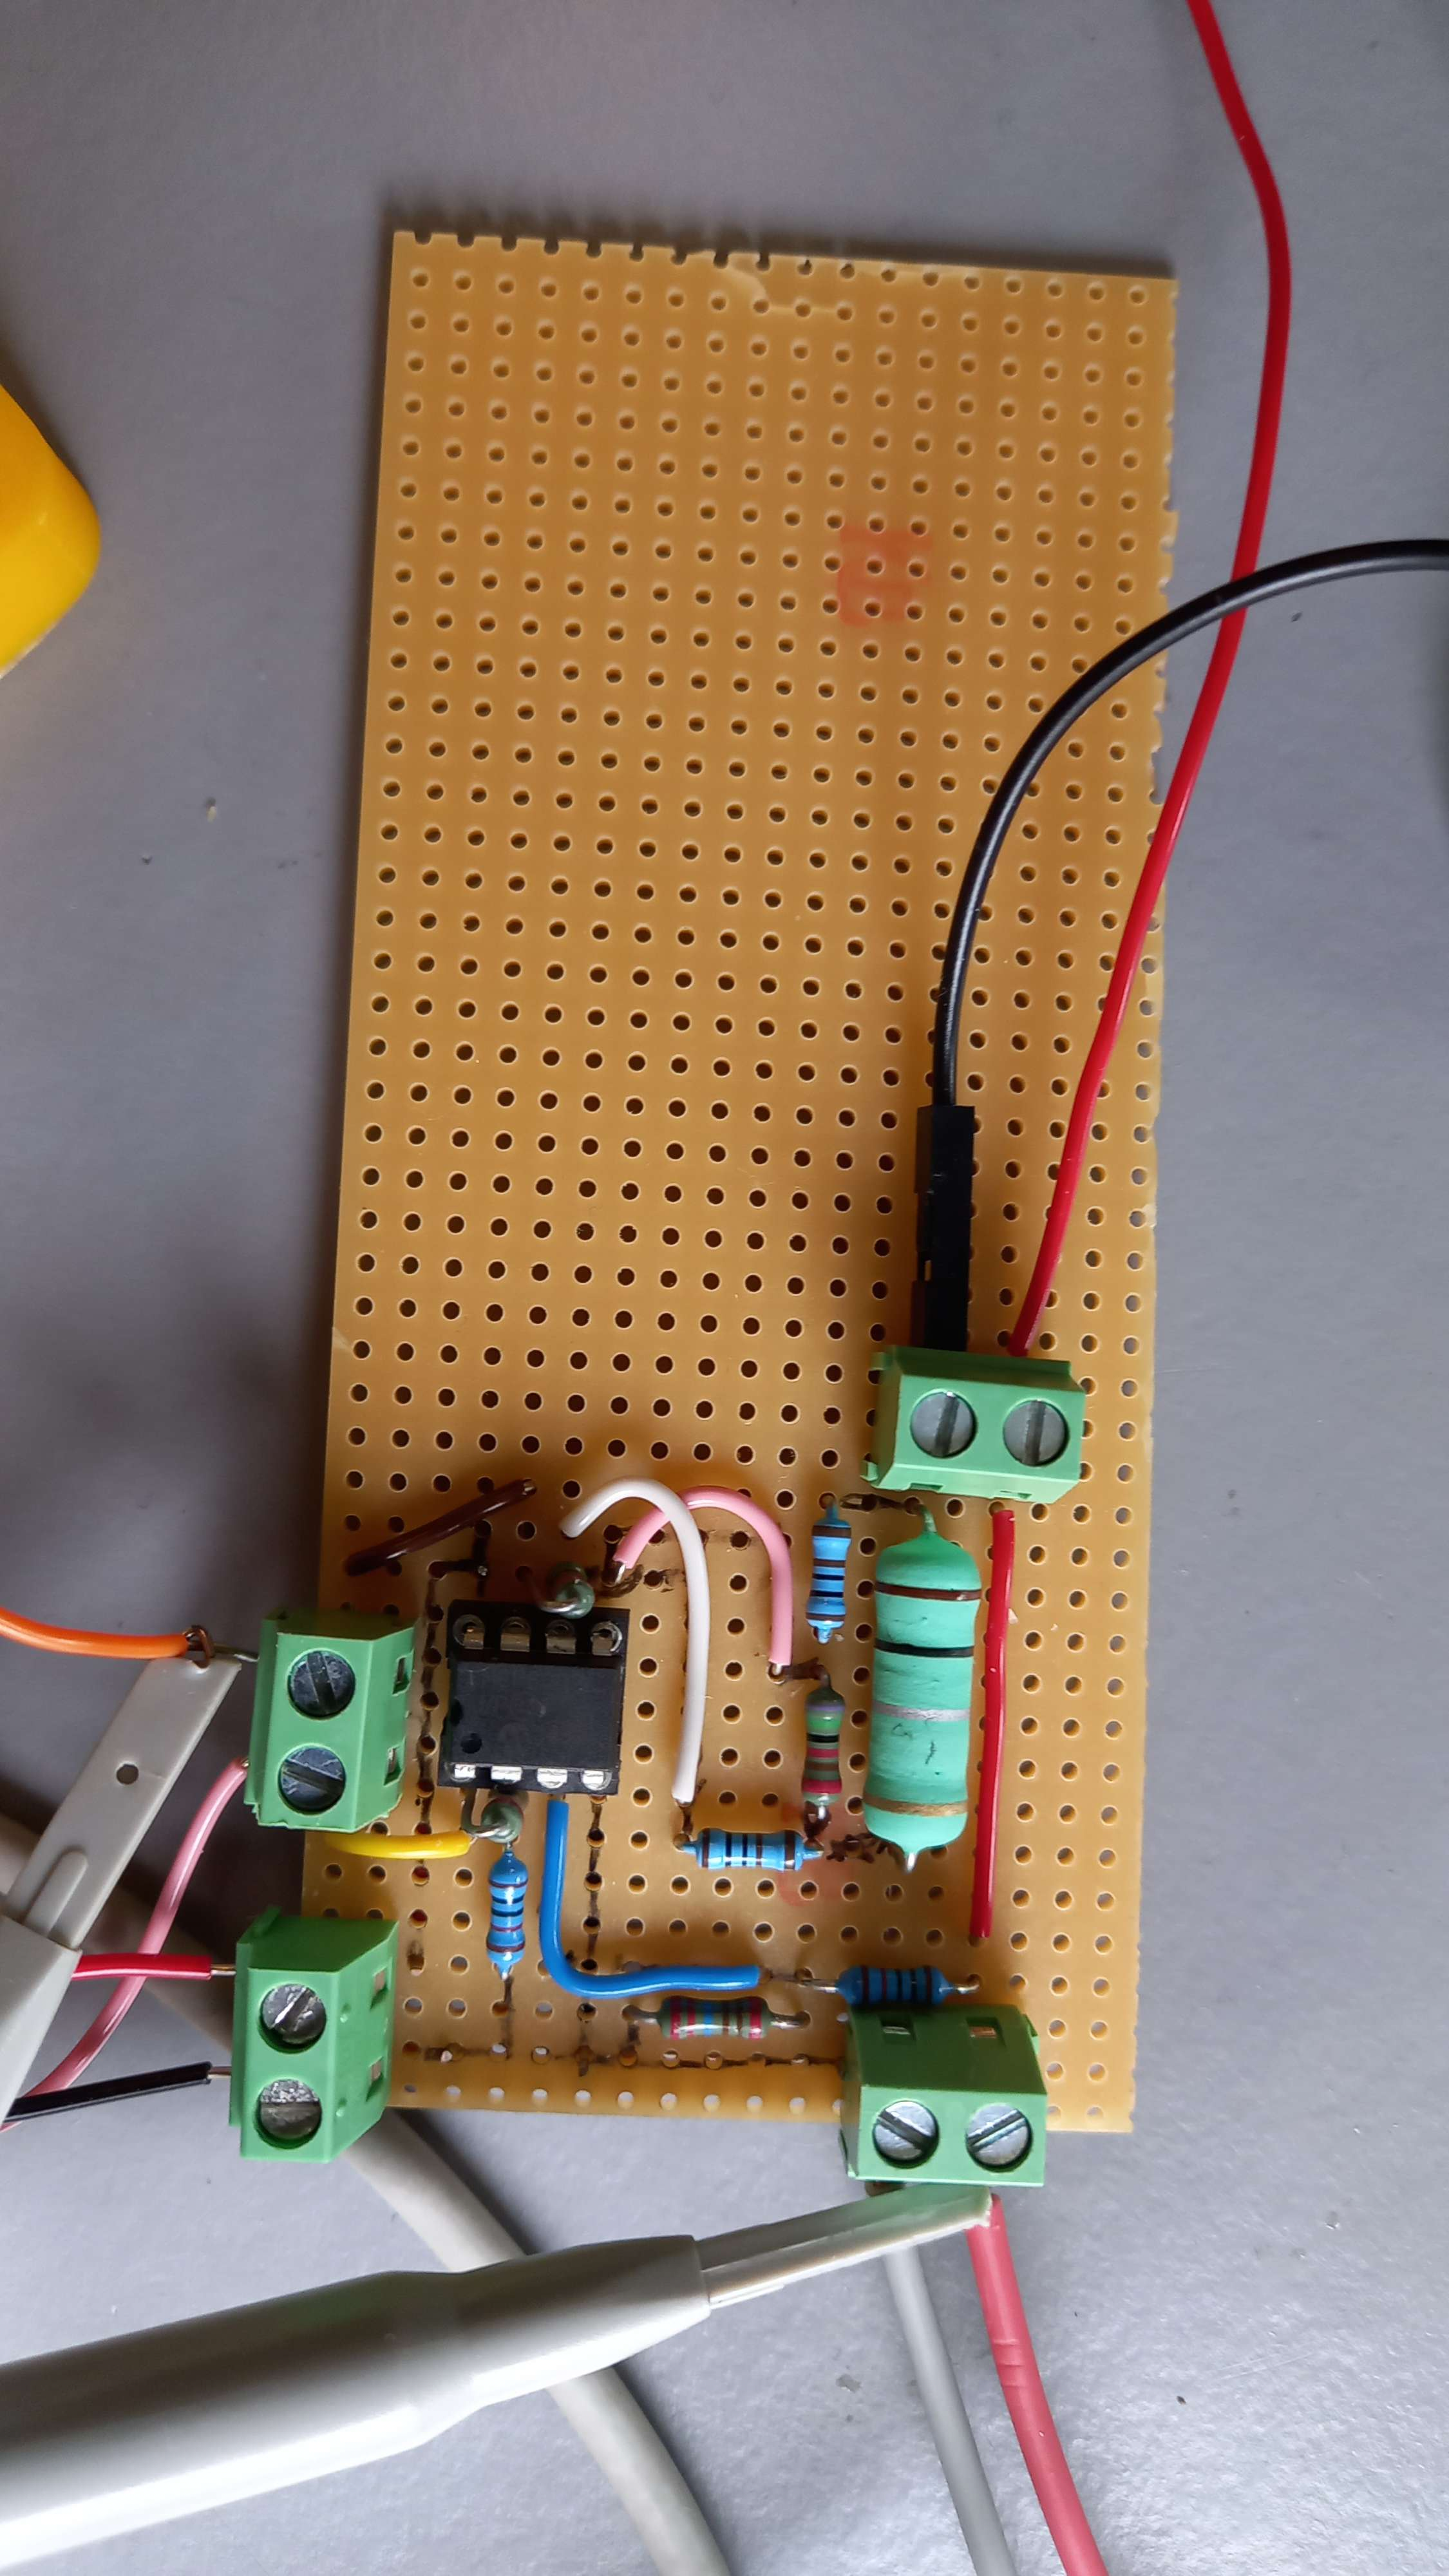
\includegraphics[scale = 0.08]{Dokumentation/Pictures/PV_strømmåler.jpg}
        \caption{Strøm/spændingsmåler til regulering af solpanelets udgangsspænding og strøm.}
        \label{pic: MPPTbuck}
        \end{figure}
        

\section{Maximum Power Point Tracking}
\subsection{Introduktion}

For at sikre kontinuerlig maksimal effekt fra solcellen anvendes et MPPT-system til at overvåge for varierende forhold og optimere systemet i realtid. Et MPPT-system gør det muligt hele tiden at opnå den størst mulige effekt fra solcellen, således at så lidt effekt som muligt går til spilde. Systemet er blevet realiseret med en Arduino, der overvåger udgangen fra solcellen og genererer et PWM-signal til en buck-konverter som derved kan justere spænding og strøm for at opnå det optimale forhold. 

\subsection{MPPT algoritme}
\subsubsection{Designovervejelser}
For at opnå maksimalt energiudbytte fra solcellen benyttes en MPPT-algoritme, som er blevet implementeret på en Arduino ATMEGA2560. Algoritmen har til formål at overvåge solcellesystemet ved at måle effekten fra solcellen, finde det maksimale effektpunkt og levere et passende PWM-signal til en buck-konverter. Der er mange forskellige typer algoritmer til at optimere energiudbyttet fra en solcelle, og i dette projekt er der taget udgangspunkt i en P \& O (Perturb \& Observe)-algoritme, som er blevet modificeret en smule.

\subsubsection{Implementering}
Arduionen modtager ADC-målinger fra solcellen, som består af en strømmåling og en spændingsmåling fra et analogt kredsløb. Ud fra dette beregner programmet effekten, husker den forrige effektværdi og finder forskellen mellem dg em. På denne måde er det muligt hele tiden at spore, hvilken vej effekten bevæger sig, og korrigere duty-cyclen på PWM-signalet til at ligge omkring et arbejdspunkt for maksimal effekt, som bruges af buck-konverteren. Algoritmen afviger fra den originale P\&O-algoritme ved ikke direkte at se på forskelle i spændingsmålinger og derudover have en variabel til at skifte retning på, hvor PWM-signalet bevæger sig hen afhængig af dens placering på den karakteristiske effektgraf for solcellen. Et flowchart for algoritmen er vist i figur \ref{fig: MPPT Flowchart}.
        
\begin{figure}[H]
 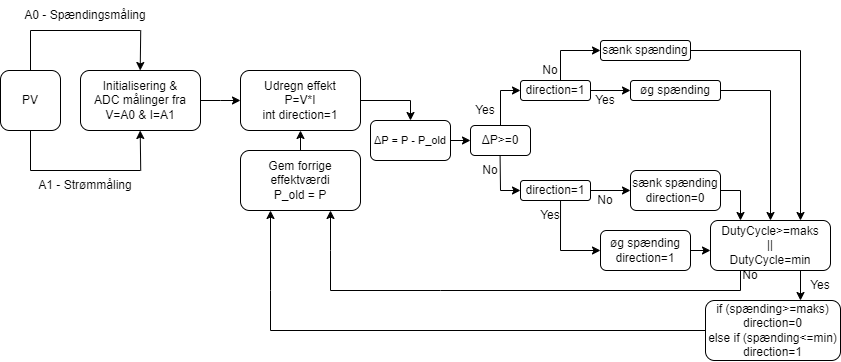
\includegraphics[width=\textwidth]{Dokumentation/mpptflowchart.drawio (1).png}
  \caption{MPPT-algoritme flowchart}
  \label{fig: MPPT Flowchart}
  \end{figure}
Undervejs er der blevet lavet mange ændringer i algoritmen og opsætningen af de forskellige elementer, der bruges i programmet. Vi er stødt på mange udfordringer mht. opsætning og behandling af analoge måleværdier, timere og generel stabilitet af systemet og har måttet bruge en del tid på at overkomme disse problemer. Der er til sidst i projektet fundet en effektiv løsning, som giver os den ønskede effekt af et MPPT-system.

MPPT-koden er vedhæftet som bilag.


    \subsection{MPPT buck}
        Dette delkredsløb kontrolleres af MPPT-algoritmen og anvendes til at regulere indgangsstrøm/spændingen fra solcellen så effekten kan tilpasses og optimeres efter det påsatte load.
        
        \subsubsection{Delkrav}

            \begin{enumerate}
                \item Skal kunne regulere forholdet mellem sin egen indgangs- og udgangsspædning samt indgangs-/udgangsstrøm som en funktion af et PWM-kontrolsignal.
                \item Skal kunne håndtere en indgangspændning på op til 23V
                \item Skal kunne håndtere en indgangsstrøm på op til 0.66A
                \item Må ikke trække mere end 20 mA fra PWM-signalet.
                \item Skal være effektiv nok til at tillade videre regulering af udgangsspændingen til 5V og herefter kunne oplade en kondensator.
                \item Skal kunne fungere ved 50kHz.
            \end{enumerate}
            
        \subsubsection{Designovervejelser}
            
            
            Switch
            I valg af switch overvejes forskellige opsætninger af switches som vist i figur \ref{fig: Switch designs}. I figuren ses de forskellige iterationer af switch opsætninger der er blevet anvendt i buck converterne i PV-delen af opsætningen. Figuren viser den første iteration af switch længst til vænstre og nyere versioner mod højre.
            \newline
            I iteration 3 anvendes opsætningen som er lavet til en P-kanal med en N-kanal MOSFET. Dette skyldes problemer med den valgte P-kanal mosfet i iteration 2 af valg af switch. Det skal noteres at selv om denne opsætning af switch er den der indgår i den endelige opsætning er dette ikke en optimal løsning da Gate-Source ON spændingen vil føre til et spændingstab på ca. 2 volt over MOSFET'en. Grundet tidsmangel er en mere optimeret opstilling som den set i iteration 4 ikke blevet implementeret.\newline
            
            \begin{figure}[H]
            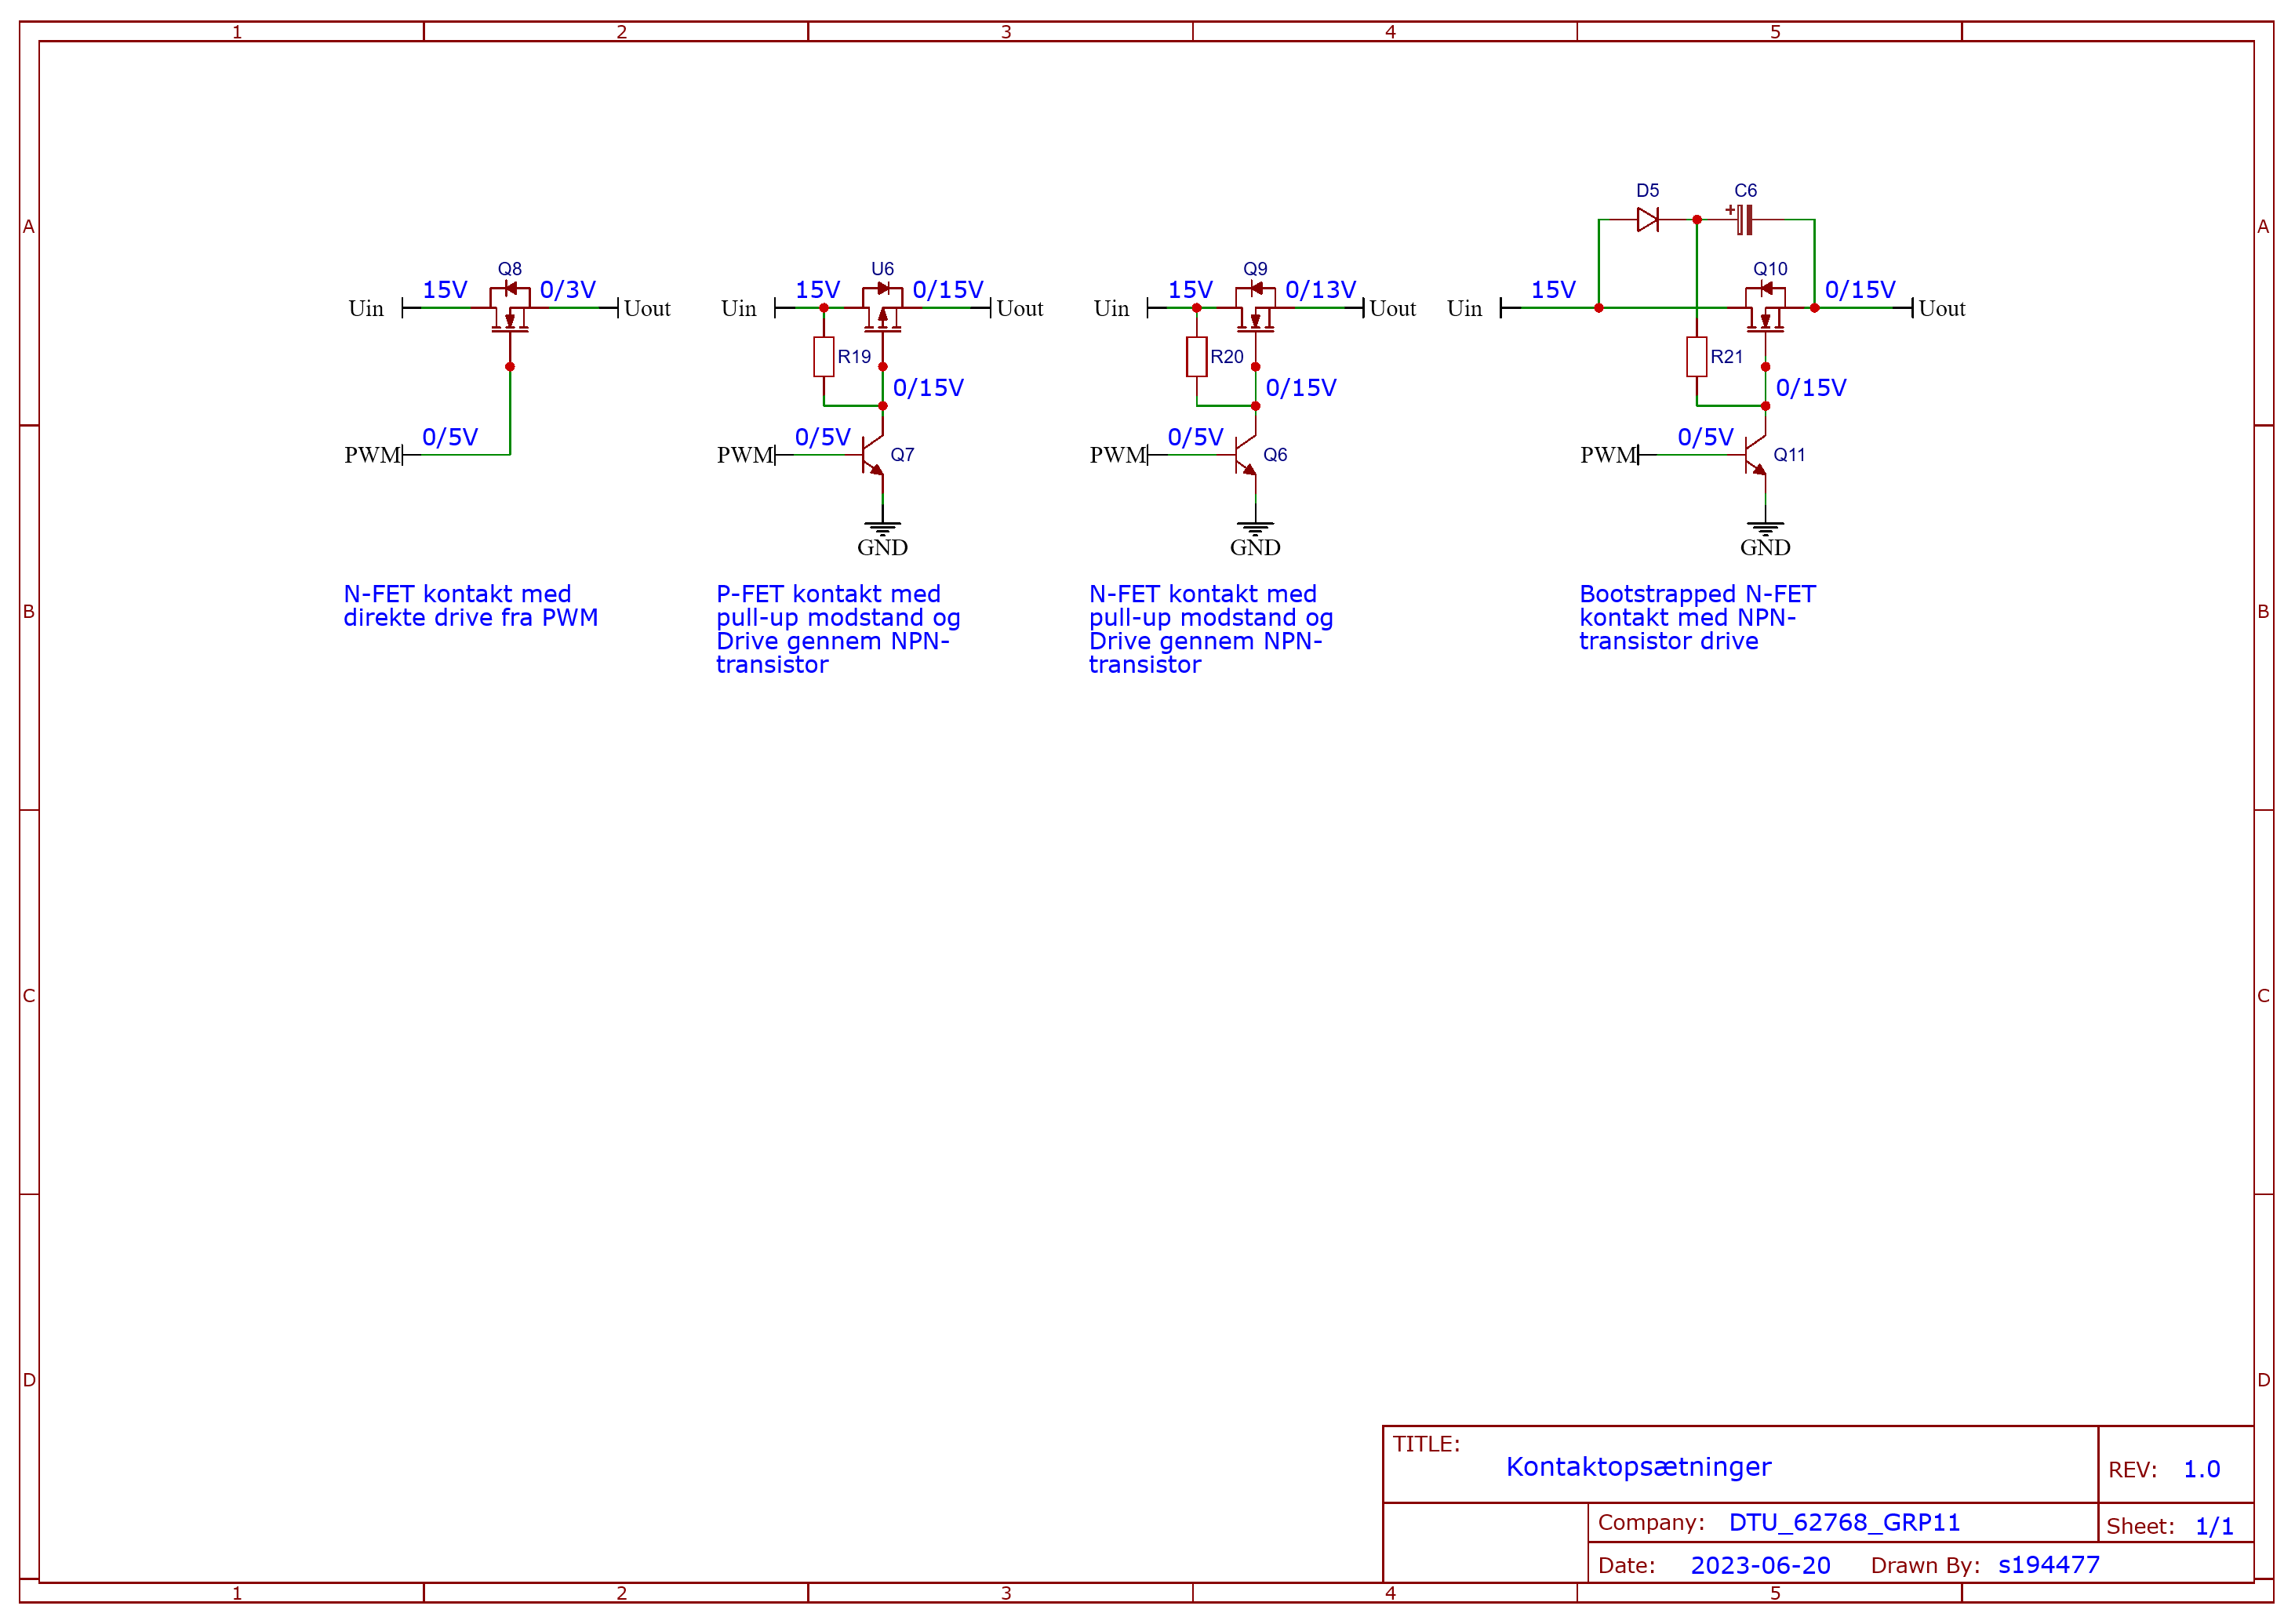
\includegraphics[width=\textwidth]{Dokumentation/Figures/PV_Converter switches.png}
            \caption{Forskellige itterationer af switch-opsætninger til buck convertere.}
            \label{fig: Switch designs}
            \end{figure}
            
            filterkomponenter:
                Følgende ligning beskriver den teoretiske udgangspænding af en buck converter i forhold til dens indgangsspænding:\newline
                $$U_{ud} = PWM \cdot U_{ind} $$\newline
                Det fremgår af dette at den gennemsnitlige udgangsspænding ikke er afhængig af filterværdierne beskrevet i følgende.
            
        \subsubsection{Implementering}

            Kondensator:
            Det fremgår af det overordnede diagram i projektbesrkivelsen (se appendix \ref{}) at der mellem MPPT'en og 5volts reguleringen i PV-grenen skal indgå en ladekondensator med en komponentværdi på 15mF. For simplificering af kredsløbbet implementeres denne ved at anvende denne kondensator som filterkondensator og denne værdi er derfor givet.
            
            Spole
            I valg af spole tages højde for at denne har en minimumsvørdi for at kunne køre i en kontinuert operationscyklus. Herudover har spolens værdi inflydelse på størelsen af de fluktiationer der ses i udgangsstrømmen, $\Delta I$.\newline

            Spoleværdien kan estimeres ud fra følgende ligning:
            $$L = \frac{1-k}{16 f^2 C}$$
            $$\rightarrow L = \frac{1-0}{16\cdot 50\cdot 10^3 Hz \cdot 15\cdot 10^{-3}F} \rightarrow 1,33nF$$
            \newline
            Ved denne værdi vil udsvingene i udgangstrømmen dog være for stor. Af denne årsag vælges en støre spoleværdi hvor den maksimale udsvinging ikke overgår 2\% af solcellens udgangsstrøm ved maksimal effekt.
            $$\Delta I_{2\%} = 0,02 \cdot I_{MP} = 0,02 \cdot 0,66A = 13,2mA$$
            $$L = \frac{U_s(1-k)k}{f\cdot \Delta I} = \frac{15 V\cdot (1-0,2)\cdot 0,2}{50\cdot 10^3 Hz \cdot 13,2 \cdot 10^{-3} A} = 3,64mH$$\newline
            
            
            Diode
            En Shotky diode tænkes at anvendes da disse har et lavere fremadrettet spændingsfald. Dette bør føre til en højere effektivitet, og en sådan diode forsøges derfor at vælges i implementeringen.

            Opbygning
            opbygningen laves på hulprint for at undgå at skade et fumlebræt ved højere effektværdier, samt for at undgå støj på signalerne. Opbygningen kan ses i billede \ref{pic: MPPTbuck}

            \begin{figure}[H]
            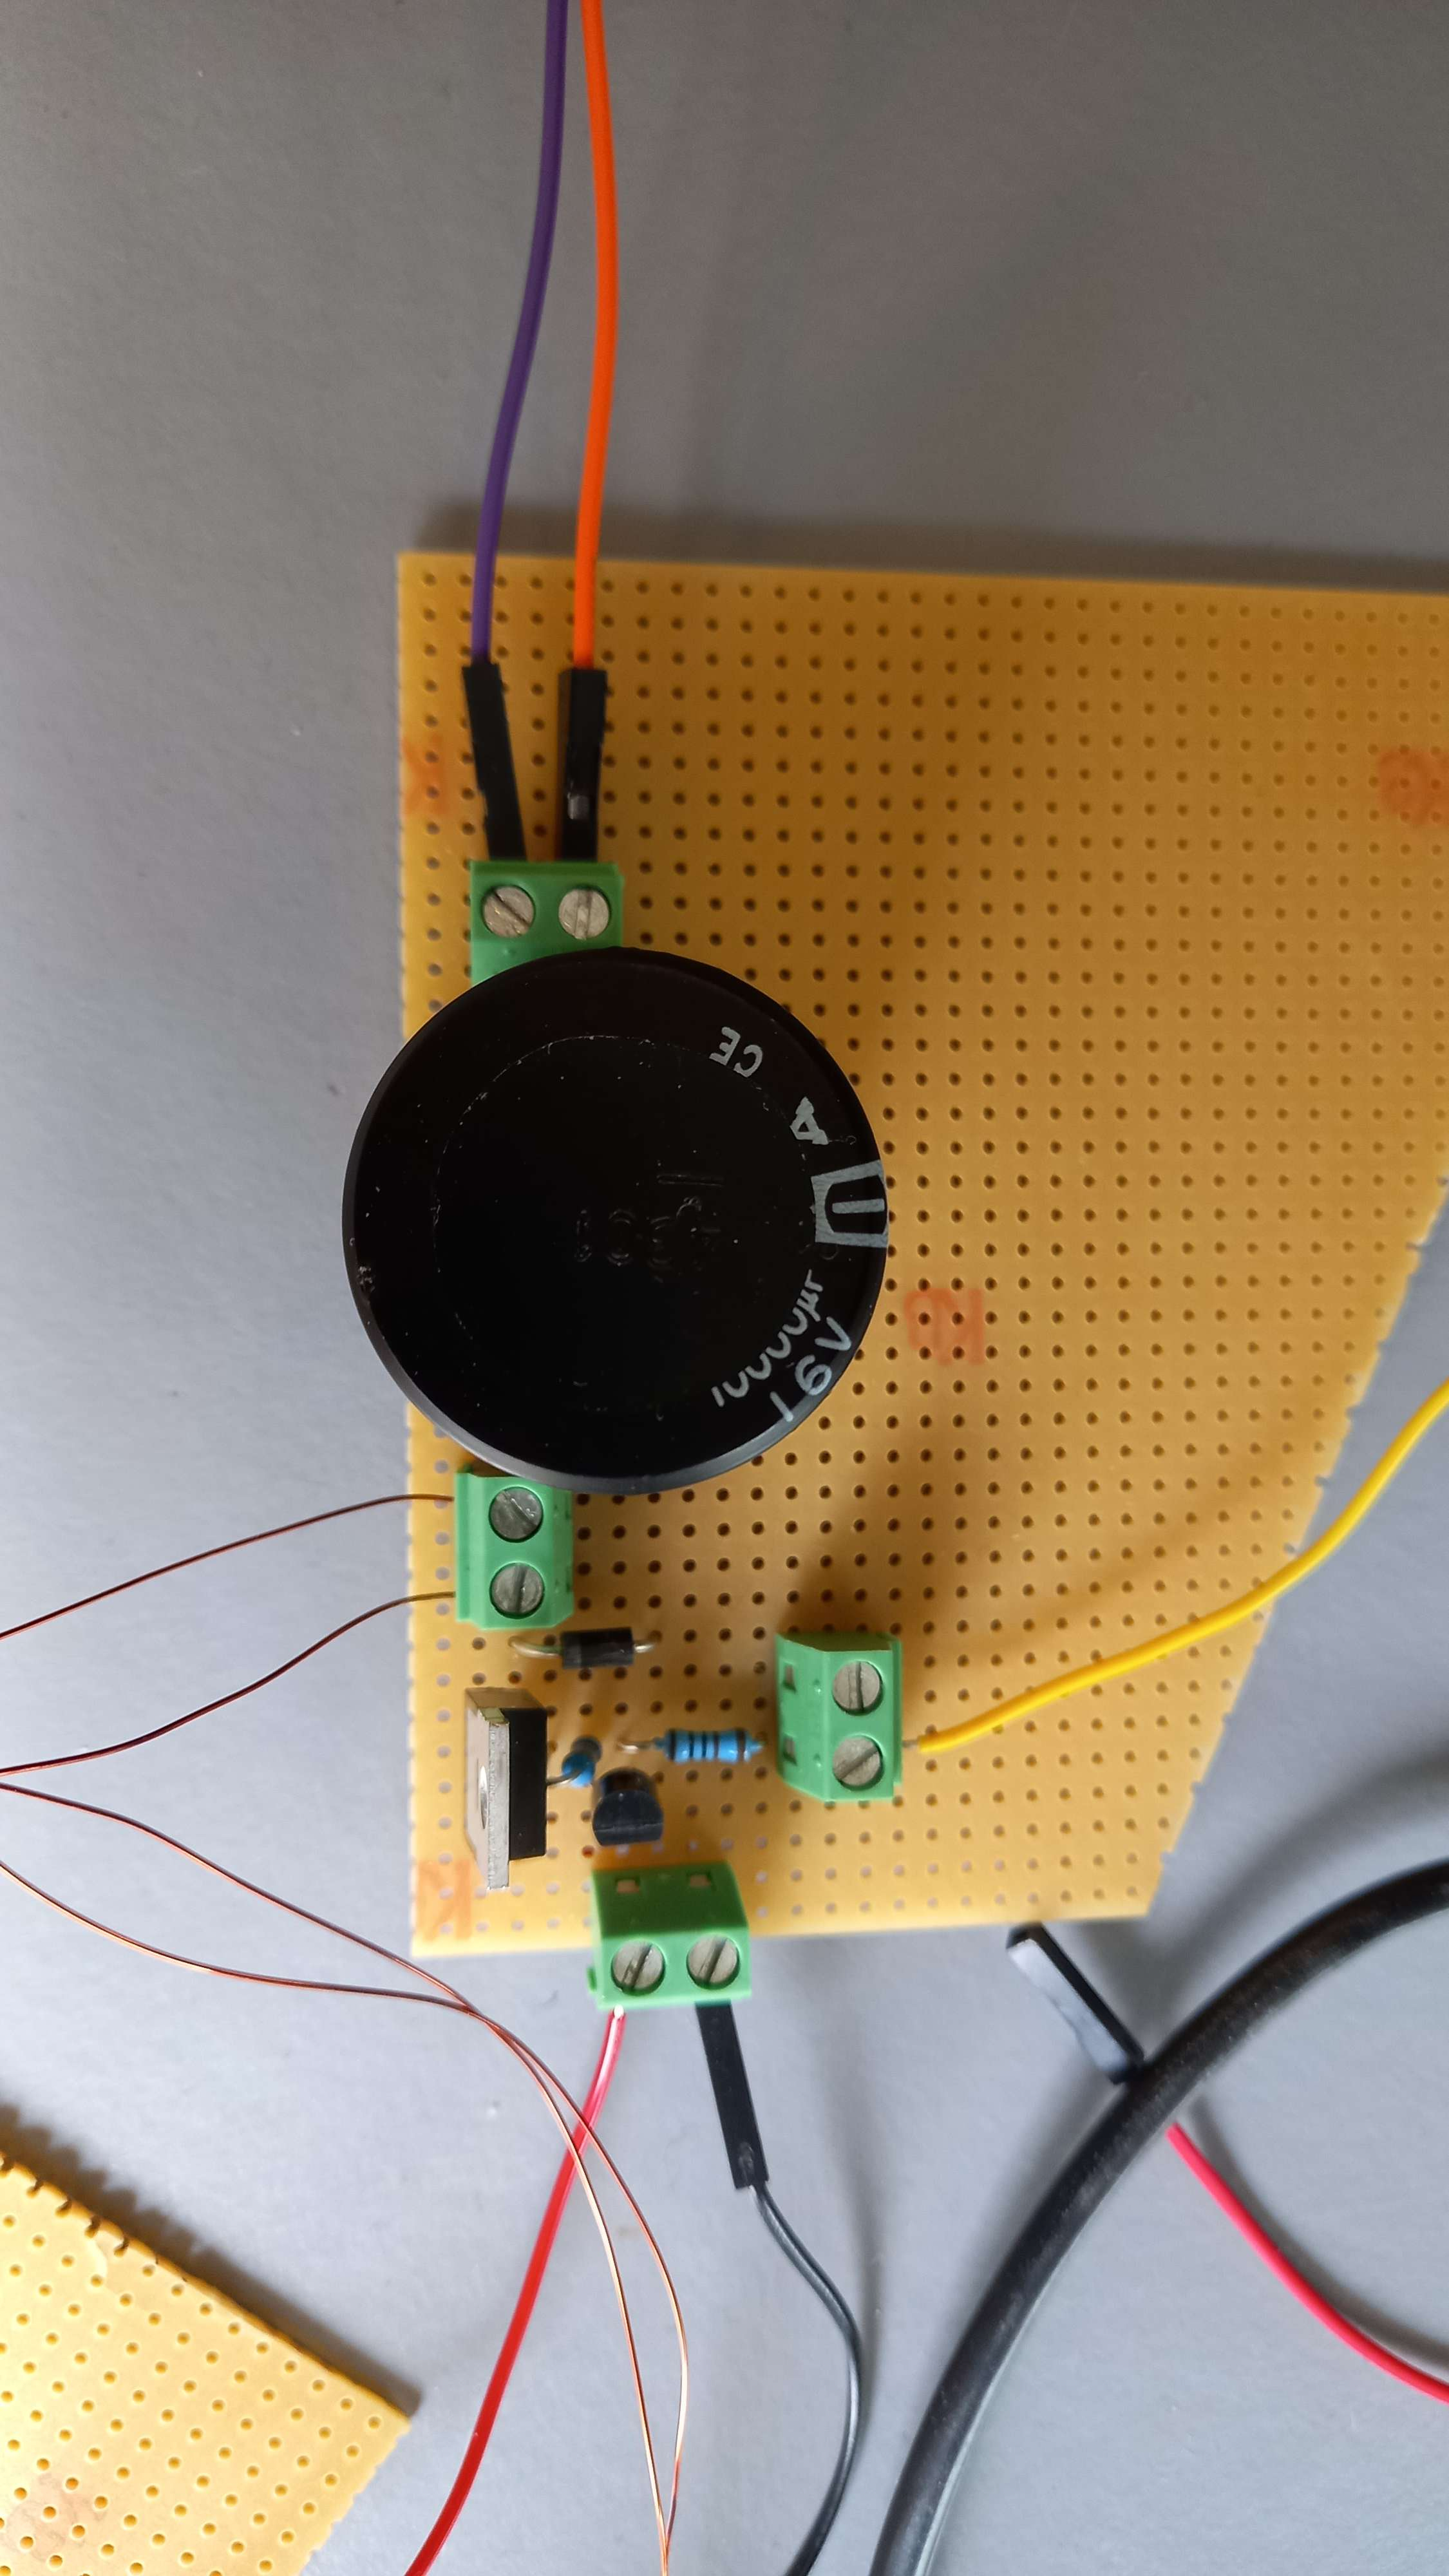
\includegraphics[scale = 0.1]{Dokumentation/Pictures/PV_MPPTbuck.jpg}
            \caption{Buckconverter til MPPT regulering af solpanel}
            \label{pic: MPPTbuck}
            \end{figure}
            
        \subsubsection{Test}
            Til test af hardwaren kobles en $68\Omega$ effektmodstand til MPPT-buckconverterens udgang, solpanelet kobles på dens indgang, og en signalgenerator anvendes til at give et 5V PWM-signal til kontrolbenet. Diverse spændinger måles da i systemet og resultaterne som ses i figur \ref{fig: Testresultater MPPT-Buckconverter} fås på baggrund heraf.\newline
            Det ses her at det er muligt, ved at variere Dutycyclen på PWM signalet, kan vi variere spændingen hen over solpanelet, den strøm det levere, samt forholdet imellem disse værdier. Det ses herudover også i "Effekt/DutyCycle"-grafen, at den leverede effekt variere som følge af den påtrykte dytycycle af PWM signalet til buckconverteren, og at denne herved kan anvendes sammen med et målesystem og en MPPT-algoritme kan optimere den leverede effekt fra solpanelet.
            
            \begin{figure}[H]
            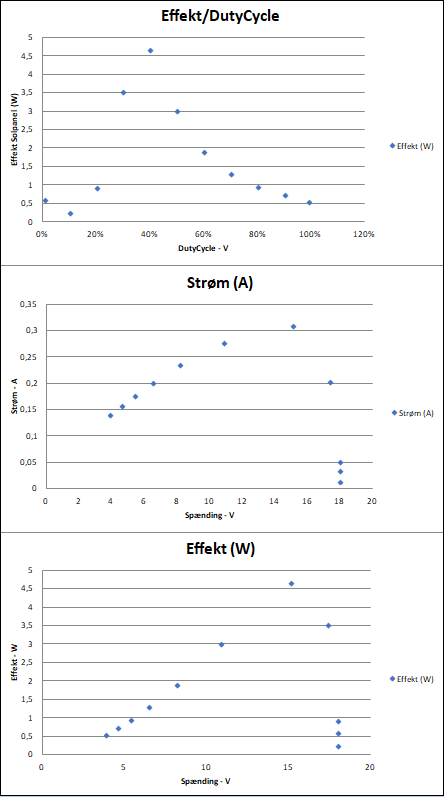
\includegraphics[scale = 0.8]{Dokumentation/Figures/PV_buckHardwareTest.png}
            \caption{Forskellige itterationer af switch-opsætninger til buck convertere.}
            \label{fig: Testresultater MPPT-Buckconverter}
            \end{figure}
                    
\section{Udgangsconverter}
        
    \subsection{Delkrav}
        Skal kunne regulere en vilkårlig spænding fra MPPT'en til 5V.
        
    \subsection{Designovervejelser}
        
        Switch
        Udgangsconverteren anvender en bootstrapped nmos switch til at drive buckconverteren. Dette gør i teorien at denne vil kunne opnå næsten samme spænding på udgangen som den har på indgangen i modsætning til den i MPPT'en anvendte buck converter der har et spændingsfald på ca. 2 Volt.
        
        Spole/Kondensator/diode
        Værdierne på spolen og kondensatoren vælges på baggrund af de samme ligninger som anvendes tidligere i afsnit 1.1.3.\newline
        resultatet er følgende opsætning som set i figur \ref{fig: 5V buck PV}
        
        \begin{figure}[H]
            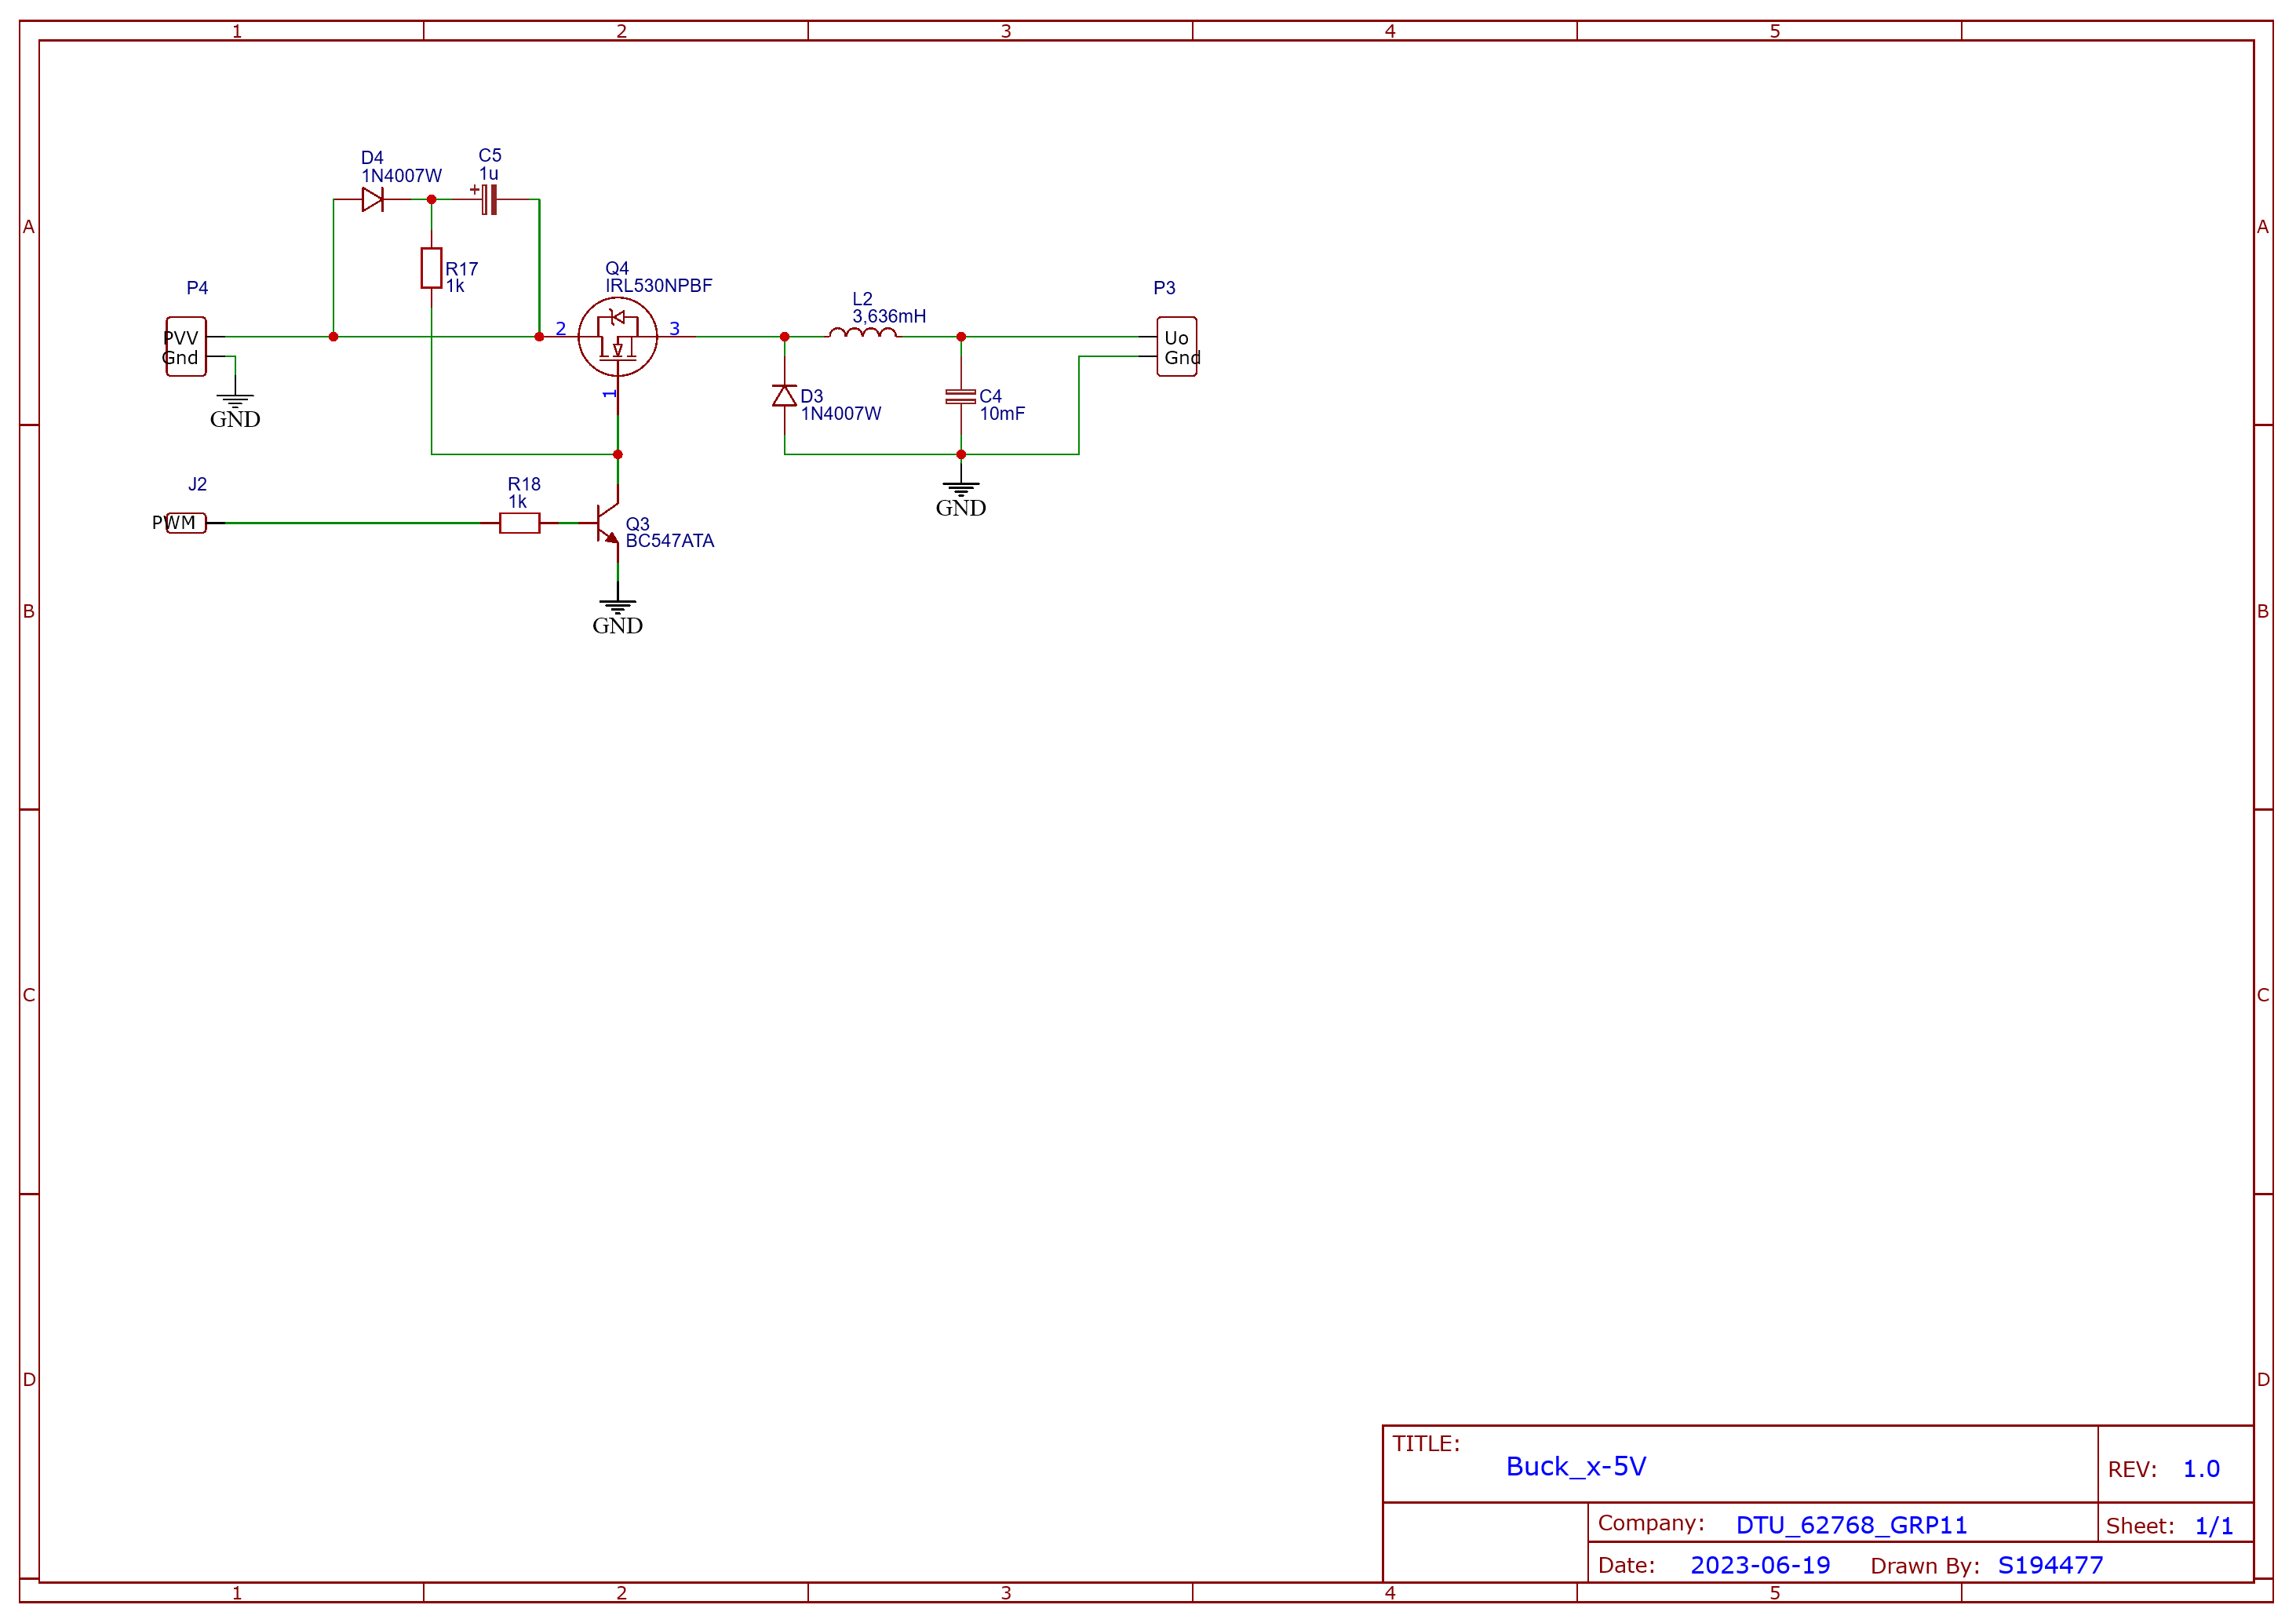
\includegraphics[width=\textwidth]{Dokumentation/Figures/PV_Buck_x-5V.png}
            \caption{Diagram over opstillingen af 5V reguleringsbuckconverteren}
            \label{fig: 5V buck PV}
        \end{figure}

            
    \subsection{Implementering}
        \begin{figure}[H]
        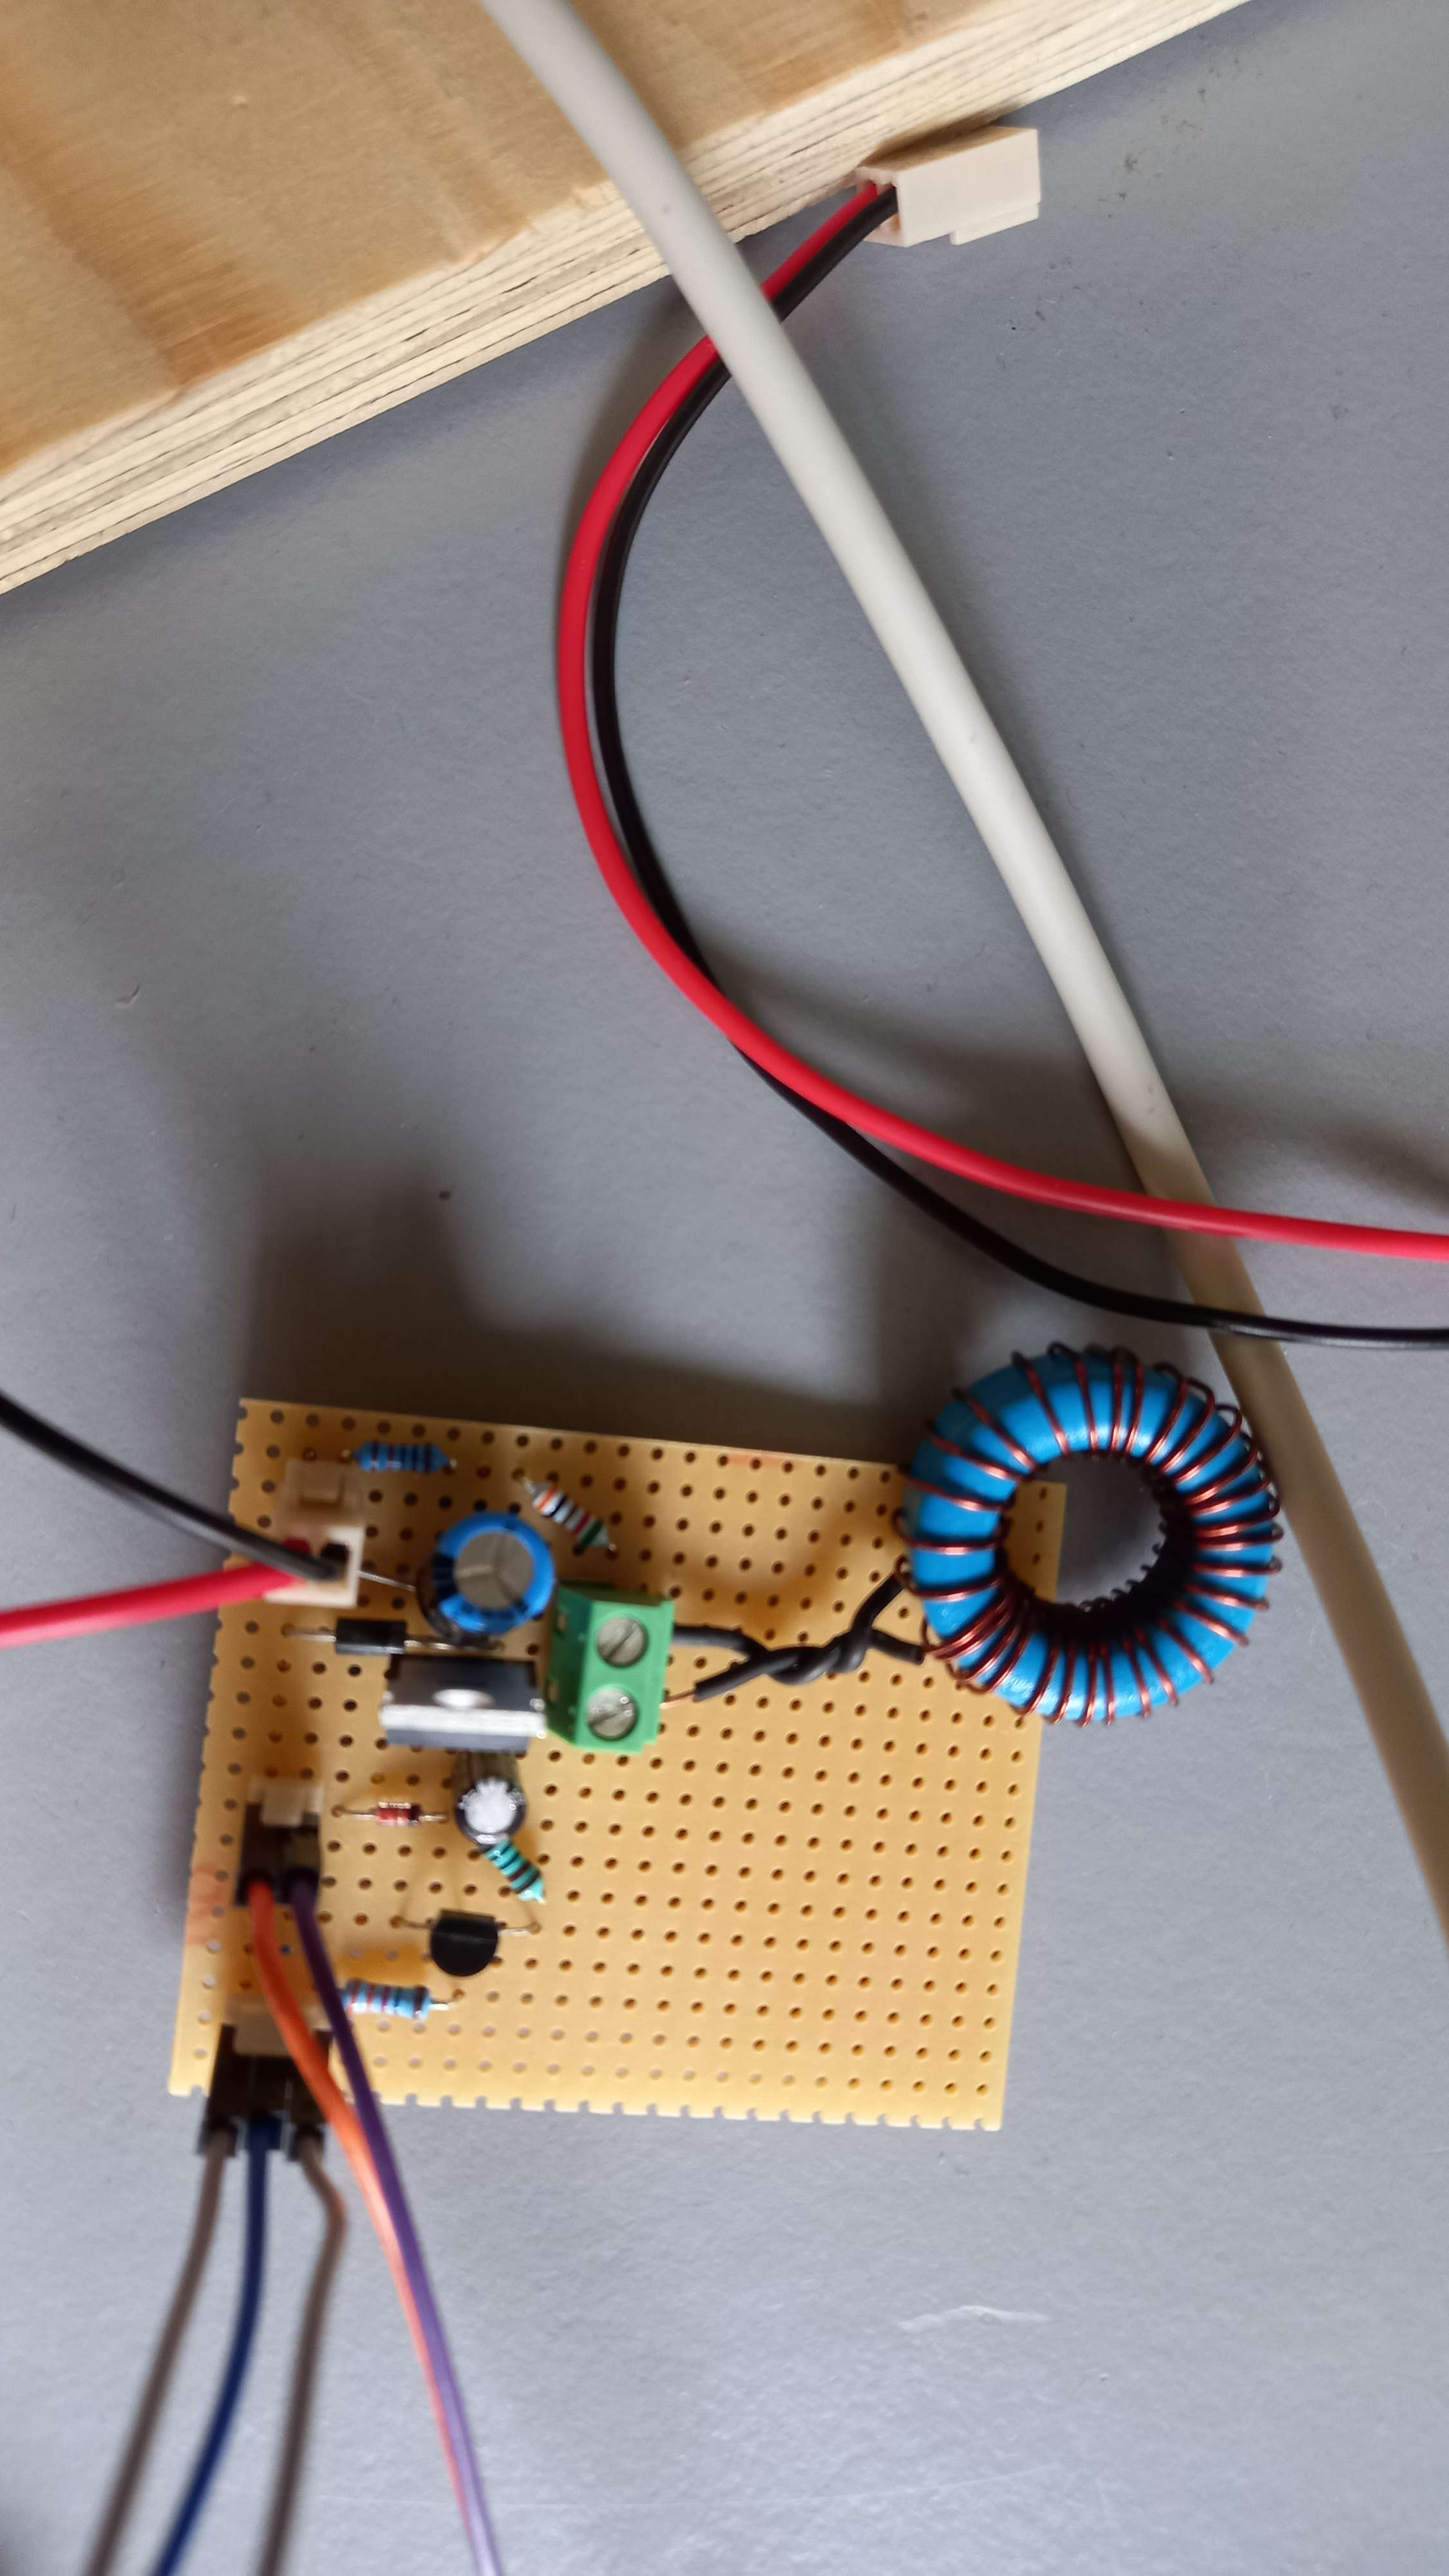
\includegraphics[scale = 0.1]{Dokumentation/Pictures/PV_udgangsbuck5V.jpg}
        \caption{Buckconverter til at regulere spændingen fra solpanelet til 5V til anvendelse af opladning af superkondesatoren}
        \label{pic: MPPTbuck}
        \end{figure}

    
    \subsection{Test}
        Som en del af den samlede funktionstest i afsnit \ref{afsnit: testafsnit} kan det ses at udgangsspændingen holdes på ca. 5V når indgangsspændingen varieres, indtil et punkt hvor solcellen ikke kan levere en høj nok effekt hvor spændingen så falder.
        

\section{Test af solcellesystem} \label{afsnit: testafsnit}

\subsection{Funktionstest}
For at lave en test på solcelle-systemet, målte vi en række værdier over forskellige loads. Grafen for solcellens spænding og strøm samt spændingen over loaden over en række forskellige load-modstandsværdier er vist nedenfor.

    \begin{figure}[H]
        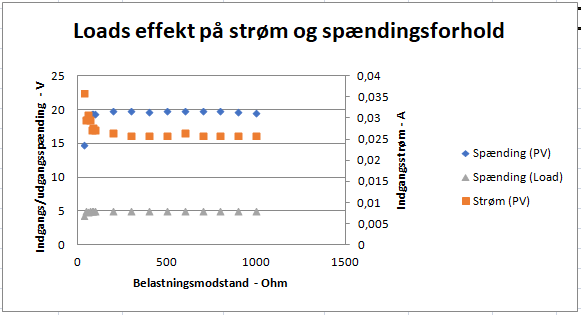
\includegraphics[width=\textwidth]{Dokumentation/Figures/PV_FuldTest.png}
        \caption{Test af solcelle-system}
        \label{fig: Test af solcelle-system}
        \end{figure}

        Diagrammet viser at spændingen bliver holdt på 5V på udgangenstrinnet over forskellige solcelle-spændinger og strømme samt forskellige loads. Og det kan konkluderes at kredsløbet fungerer som ønsket og i henhold til kravspecifikationerne.

\subsection{Effektivitetstest}
For at teste effektiviteten af convertersystemet til solpanelet måles den leverede strøm fra solpanelet til systemet, samt strømmen gennem en varierende belastningsmodstand. Herudover måles spændingsfaldet over modstanden, samt spændingen over solpanelets to terminaler. Dette anvendes til at udregne effekten leveret af solpanelet, samt effekten leveret til belastningen, og videre udregnes forholdet mellem effekten leveret til belastningen, samt effekten leveret fra solpanelet 
for at finde effektiviteten af systemet. Resultaterne af denne test kan ses i figur \ref{}    
    \begin{figure}[H]
        \includegraphics[width=\textwidth]{Dokumentation/Figures/PV}
        \caption{Test af solcelle-system}
        \label{fig: Test af solcelle-system}
        \end{figure}

        
\end{document}